\chapter{Implementace}
\definecolor{tableGreen}{rgb}{0.53, 0.66, 0.42}
\definecolor{tableOrange}{rgb}{1.0, 0.6, 0.4}
\definecolor{tableRed}{rgb}{1.0, 0.44, 0.37}

\label{implementace}
Obsahem této kapitoly je popis jednotlivých fází implementace. Je zde popsáno, jakým způsobem byly zpracována data potřebná pro funkčnost aplikace. Následně tato kapitola obsahuje způsob řešení jednotlivých částí, které pokrývají hlavní funkce aplikace, jako jsou zpracování vstupního souboru a navazování matrik na záznamy. V~jednotlivých fázích jsou také vypíchnuty nejdůležitější problémy, na které bylo naraženo a jejich řešení.

\section{Příprava dat}
\subsection{Území České republiky}

Jelikož má být aplikace schopná pracovat i s~územím bylo nutné zpracovat územní celky v~rámci České republiky. Tyto celky jsou popsány pomocí RUIAN\footnote{RUIAN -  \url{https://www.cuzk.cz/ruian/Poskytovani-udaju-ISUI-RUIAN-VDP/Ciselniky-ISUI.aspx}} číselníků ISÚI, které v~sobě obsahují následující informace:
\begin{itemize}
	\item \textbf{RUIAN kód} - číselná identifikace v~rámci typu území
	\item \textbf{Název} - řetězec označující území
	\item \textbf{Kód nadřazeného území} - číselná identifikace území, nacházejícího se o~jeden stupeň v~hierarchii výše
	\item \textbf{Od} - datum od kdy jsou tyto informace platné
	\item \textbf{Do} - datum do kdy jsou tyto informace platné
	\item \textbf{Datum vzniku} - datum přidání informací do číselníku
	\item \textbf{Ostatní} - informace specifické ke konkrétnímu typu území
\end{itemize}

Pro každý typ území bylo tak zpracováno 7 číselníků od státu až po části obcí. K~zpracování číselníků byl napsán shell skript, který číselníky zformátoval do podoby SQL skriptu. Ke každému území byla přiřazena číselná hodnota označující typ území od 0 do 5. Části obcí a městské celky byly zařazeny do stejného typu 5 (viz tabulka \ref{tabulka_typy}). V~databázi nebyly RUIAN kódy použity jako primární klíč tabulky území, protože nebyly v~rámci celku unikátní (pouze v~rámci typu). Z~tohoto důvodu byl napsán Python skript, který navázal území na jejich nadřazené celky za pomocí identifikačního čísla uděleného v~rámci databáze a také upravil SQL skript aby obsahoval tyto hodnoty.

\begin{table} \label{tabulka_typy}
	\centering
	\begin{tabular}{ll}
		\hline
		\textbf{Číselný typ území} & \textbf{Název typu území} \\ \hline
		\textbf{0} & Stát \\ 
		\textbf{1} & Regiony \\ 
		\textbf{2} & Kraje \\ 
		\textbf{3} & Okresy \\ 
		\textbf{4} & Obce \\ 
		\textbf{5} & Části obcí \\ 
		\textbf{5} & Městské celky \\ 
	\end{tabular}
	\caption{Zjednodušené rozdělení území ČR na typy}
\end{table}

\subsubsection{Zeměpisné souřadnice}
Důležitou součástí zpracování území bylo přiřadit k~jednotlivým celkům souřadnice. Získání souřadnic bylo docíleno pomocí web scrapingu\footnote{web scraping - sběr dat z~webových stránek} v~jazyce Python. Skript souřadnice získával z~webu Wikipedie, kde každá obec a její části mají vytvořenou stránku, na které se nachází odkaz na web GeoHack\footnote{Geohack - \url{https://geohack.toolforge.org/}}. Zde jsou pro každé území uložené souřadnice v~podobě zeměpisné šířky a délky. Tyto souřadnice v~decimální podobě skript přidává k~vytvořenému SQL skriptu, tak aby mohli být uloženy v~databázi. Vyhledávání na webu Wikipedie probíhalo pomocí zadání názvu a RUIAN kódu území. Jestliže se jednalo o~část obce nesoucí stejné jméno jako její nadřazená obec, pak byly i jejich souřadnice stejné. Souřadnice museli být otestovány na výskyty duplicitních hodnot pro území, které spolu neměli nic společné a v~těchto případech manuálně opraveny.

Souřadnice pro území jiných typů než 4 a 5 nebylo potřeba zpracovat, protože v~aplikaci pracujeme hlavně s~dříve zmíněnými typy území.

Díky zpracování souřadnic všech potřebných celků bylo možné namapovat sousedy jednotlivých území do okruhu 5 km a tuto mapu uložit do databáze pro příští využití, tak aby se vzdálenost nemusela pokaždé vypočítávat. Vzdálenost mezi územími byla počítána pomocí Haversinova vzorce \cite{Haversine}:

\begin{equation} \label{Haversinův vzorec}
	d = 2*r*arcisn(\sqrt{sin^2(\frac{\varphi_{2} - \varphi_{1}}{2})}+cos\varphi_{1}*cos\varphi_{2}*sin^2(\frac{\lambda _{2} - \lambda_{1}}{2}))
\end{equation}

 
kde d je vzdálenost mezi dvěma body, r je poloměr země v~kilometrech (6371 km), $\varphi_{1}$, $\varphi_{2}$ jsou souřadnice zeměpisných šířek a $\lambda_{1}$, $\lambda_{2}$ zeměpisných délek bodů 1 a 2 v~desetinných hodnotách. Funkce, která pracuje s~daným vzorcem byla převzata z~webu GeeksforGeeks~\cite{Haversine_function}. Při testování je možné narazit na pár odchylek, které jsou však v~našem případě naprosto zanedbatelné.

\subsection{Matriky}
\subsubsection{Extrakce dat}
Bylo zapotřebí zpracovat archivy uchovávající digitalizované matriční knihy. Jejich zpracování bylo docíleno opět pomocí web scrapingu v~jazyce Python. Muselo být napsáno osm skriptů, "scraper\_NAZEVMESTA.py", jelikož každý archiv měl jinou strukturu. 

Nejdříve proběhla analýza struktury webu, zkoumání elementů, které uchovávají důležité informace. Každý web měl seznamy matrik zobrazené pomocí tabulkových elementů, mezi kterými se přecházelo přes stránkování. Bylo zapotřebí tedy nejdříve získat odkazy na jednotlivé detaily matrik z~těchto tabulkových elementů přes všechny jejich stránky. Některé archivy neměli možnost zobrazit matriky všech typů zároveň a bylo tedy zapotřebí procházet přes všechny tabulky všech typů. Zpracování odkazů skripty provádí po spuštění se vstupním argumentem "links" a jejich výstupem je soubor obsahující jednotlivé odkazy po řádcích. Z~tohoto souboru se pak čerpá při zpracovávání jednotlivých matrik.

Při zpracování konkrétní matriky jsou pro účely aplikace důležité jen určité informace. Matriky byly s~těmito informacemi uloženy do souborů formátu JSON pro každý archiv zvlášť. 

Nejdůležitější informací je uzemní rozsah matriky. Tedy jaké obce a části obcí tato matrika pokrývá. Pokud je zde uveden, pak je pro nás důležitý i okres, pod kterým působí, a~to pro jasnou identifikaci obcí kvůli duplicitě jmen. Do souboru JSON jsou území ukládány do pole, kde klíčem je název území a hodnotou slovník obsahující dodatečné informace o~území, které archiv poskytuje. Další důležitou informací je obsah matriky a jeho časový rozsah. Tedy jaký typ události je v~matrice zapsán a v~jakém časovém rozmezí. Typy událostí jsou v~souboru JSON označovány písmeny N (narození), Z~(zemřelí), O~(oddáni) a u~každého typu je uveden časový rozsah. V~případě indexů je postup stejný jen se pro označení používají zkratky I-N, I-Z, I-O. Pokud archiv neuvádí časové rozsahy pro jednotlivé typy, pak je každému typu přiřazen obecný rozsah matriky. Mezi ostatní důležité informace pak patří původce, signatura a inventární číslo, které pak aplikace používá jako identifikaci matrik pro uživatele.

\subsubsection{Přiřazení území}
\label{uzemi_assign}
Soubory JSON, které vznikly při extrakci dat z~archivů, bylo zapotřebí ještě upravit. Konkrétně bylo potřeba namapovat území uvedené u~jednotlivých matrik na konkrétní územní prvky obsažené v~databázi aplikace. 

Způsob jakým archivy zapisují území k~matrikám je popsán metodikou popisu matrik, kterou zveřejnilo Ministerstvo vnitra České republiky \cite{metodika}. Podle této metodiky mohou být lokality vyplněny dvěma hlavními způsoby. V~případě, že se matrika vztahuje ke všem částem nějaké obce mohou být vypsány buďto všechny části této obce nebo jen název dané obce. Druhý způsob zápisu vytváří problém, protože je potřeba aby při využití daného zápisu archivy uváděli u~jednotlivých území i jejich typ. Pokud tomu tak není je velmi obtížné rozeznat jestli je myšlena obec jako celá nebo pouze její stejnojmenná část. Dalším problémem s~touto metodikou je, že ne všechny archivy ji zcela dodržují a při zkoumání jednotlivých archivů se narazilo na případy kdy byla uvedena jak obec, tak i některá její část, a to i přestože uvedení dané obce automaticky zahrnuje i tu zmíněnou část. Z~těchto důvodů se území mapují 1:1 k~jejich uvedenému typu a neprovádí se zahrnutí částí v~případě uvedení území typu obec. Dané zahrnutí se řeší až v~kapitole popisující navazování matrik k~záznamům \ref{matcher}. Postup přiřazování území se lišil pro jednotlivé archivy a je popsán v~následujících odstavcích.

Jestliže byly územní prvky v~archivech uváděny pomocí hierarchie (část obce, obec, okres) pak se dalo území jednoznačně určit i v~případě duplicitních jmen. Výjimkou byly pouze obce Březina, nacházející se v~okrese Brno-venkov, jelikož se jedná o~speciální případ, kdy se nachází dvě stejnojmenné obce ve stejném okrese. Zde bylo zapotřebí přiřadit matriky manuálně. Výhodou tohoto zápisu také bylo, že u~každého území byl známý jeho typ. Mezi takové archivy patří Opavský, Litoměřický, Brněnský a archiv Hradce Králové.

Pouze jediný archiv uváděl u~území jejich identifikační RUIAN kód a tím byl Třeboňský archiv. Zde bylo tedy přiřazení nejjednodušší, jelikož se díky tomuto kódu hned vědělo, o~který územní prvek se jedná i jaký je jeho typ. 

Jestliže ovšem archivy neuvedly ani RUIAN kód a ani žádnou územní hierarchii musel být zvolen jiný postup přiřazení území. Mezi takové archivy patřily Středočeský a Plzeňský. Pro tyto archivy byla vytvořena mapa okresů, které pokrývají, a okresů, které s~těmito okresy sousedí. Sousední okresy byly uvedeny z~důvodu lokalit vyskytujících se na hranicích okresů. Tímto způsobem byl zúžen územní rozsah a odpadly tak některé duplicitní názvy. Postup se pak nadále u~těchto dvou archivů lišil. 

U~Středočeského archivu byly všechny uvedené území typu část obce a vždy zde byl uveden původce a okres, ve kterém se původce nachází. Díky tomu se dalo území jednoznačně určit za pomocí souřadnic na základě vzdálenosti mezi odhadovaným územím a původcem. V~případě duplicitních názvů bylo tedy zvoleno to území, které se nacházelo nejblíže k~původci.

Určování u~Plzeňského archivu bylo nejtěžší jelikož na rozdíl od Středočeského zde nebyl uveden okres původce. Jestliže se tedy dal původce jednoznačně určit, pak se dali opět na základě souřadnic určit i ostatní území. Pokud ovšem nebylo možné původce určit, určili se ostatní jednoznačně vypsané území, z~jejichž souřadnic se vypočítal centroid, který nám nahradil původce, a na základě kterého jsme pak určili ostatní nejednoznačné území. Plzeňský archiv také neuváděl jakého typu je dané uvedené území a tak v~případě, že nešlo určit jestli je myšleno území jako obec nebo jako jeho stejnojmenná část byla zvolena část. Obec byla zvolena pouze v~případě, že k~sobě uvedená obec neměla stejnojmennou část, tak jako je tomu například u~obce Plzeň. Tento postup byl odůvodněn zkoumáním archivu a zjištěním, že v~mnoha případech kde se nedalo rozhodnout o~typu zde byla uvedena i jiná část spadající do stejné obce a dle výše zmíněné metodiky by to tedy znamenalo, že i nejasné území by pak mělo být myšleno jako typ část obce.

Pokud bylo území určeno, tak k~němu v~JSONu byl připsán jeho RUIAN kód, typ označený číselnou hodnotou, souřadnice pomocí zeměpisné šířky a délky, název okresu a případně i název obce (pro území typu 5), pod kterou území spadá.

Ne všechny území se dalo přiřadit na území v~rámci naší databáze. U~matrik mohli být totiž uvedeny i zaniklé území, příliš malé územní prvky (ulice, ZSJ\footnote{ZSJ - základní sídelní jednotka}, kostely, ...) a nebo i území z~ciziny. V~případech kdy jsme tedy nebyli schopni určit území mu byla přiřazena hodnota RUIAN jako -1.

Finální verze souborů JSON po přiřazení území tedy pak vypadá takto:

\begin{small}
\begin{verbatim}
{
    "url": "https://digi.archives.cz/da/permalink?xid=29e3f91ac933f2f4",
    "puvodce": "Pavlovice u Přerova, římskokat. f. ú.",
    "signatura": "Př XI 64",
    "invCislo": null,
    "typ": "katolická",
    "jazyk": null,
    "rozsah": "1947 - 1949",
    "obsah": [
    "O•1947-1949"
    ],
    "uzemi": {
        "Pavlovice u Přerova": {
            "typ": 4,
            "ruian": 516694,
            "latitude": 49.469425,
            "longitude": 17.547772,
            "okres": "Přerov",
            "varianty": []
        }
    },
    "okresy": [
    "Přerov"
    ]
}
\end{verbatim}
\end{small}
\begin{lstlisting}[caption={Ukázka zpracované matriky ve formátu JSON z~Opavského archivu. Jedná se o~matriku oddaných v~rozmezí let 1947 až 1949. Tato matrika pokrývá jediné území, Pavlovice u~Přerova, obec v~okrese Přerov.},captionpos=b]
\end{lstlisting}

\subsubsection{Zpracování dat}
Připravené soubory JSON pak zpracovával implementovaný Python skript, který pro jednotlivé matriky vytvořil příslušné záznamy do tabulky matrik v~databázi. Zároveň tento skript vytvořil záznamy do propojovací tabulky reflektující vazbu mezi územím a matrikou pro přiřazené území. Nepřiřazené území ignoroval.
\section{GEDCOM parser}
%u "python-gedcom" dat odkaz na pouzite technologie
%tvar DATA odkaz na popis gedcom formátu
K~zpracování souborů, které uživatel nahraje prostřednictvím aplikace slouží skript "gedcom\_parser.py"\  napsaný v~jazyce Python. Tento skript se stará o~zpracování všech osob a rodin zapsaných v~nahraném souboru, kontrolu validity informací a vytváření záznamů v~případě nevalidní informace. Využívá k~tomu knihovnu "python-gedcom". Skript prostřednictvím knihovny prochází přes jednotlivé osoby/rodiny v~souboru a získává o~nich informace. Při zpracování osoby se kontroluje celistvost událostí narození a úmrtí, u~rodin událost oddání. Nejdřív je zkontrolován formát data, tudíž jestli je datum zapsáno a zdali je ve správném tvaru. Následně je kontrolováno místo, ke kterému je událost připsána. U~míst mohou nastat 3 typy situací. Místo nemusí být uvedeno vůbec a tím pádem je událost nevalidní, nebo je místo uvedeno a jednoznačně přiřazeno, a v~tomto případě je událost validní. Poslední situace, jež může nastat je, že řetězec u~místa není prázdný, ale buďto jsme k~němu nenašli v~databázi území nebo jsme jich našli více a nemůžeme ho jednoznačně určit. Pokud nastane poslední situace, tak může být informace obsažená v~řetězci jak validní tak nevalidní. Jestliže by se jednalo o~místo z~ciziny, zaniklé místo nebo příliš malý územní prvek, pak by byla informace validní a místo by se pouze nenacházelo v~databázi. Zároveň se ale může jednat o~poznámku nebo nesmyslný řetězec kdy by se jednalo o~nevalidní informaci. V~takové situaci skript nerozhoduje validitu informací. Ta je rozhodnuta až prostřednictvím aplikace samotným uživatelem. Osoby a rodiny, ke kterým se řetězec obsažený v~tagu místa vztahuje, jsou tak podle tohoto řetězce sdružovány za pomocí pythonovského slovníku. To z~toho důvodu, aby se pak uživatelem zvolené místo mohlo přiřadit ke všem osobám/rodinám, kterých se místo týká.

U~události úmrtí je vhodné ještě zmínit, že pokud známe věk osoby, tedy známe její rok narození, a víme, že je osoba mladší 100 let, pak v~případě, že zde není událost úmrtí uvedena, ji neprohlašujeme za chybějící. Pokud ale nejsme schopni zkontrolovat věk osoby, pak automaticky říkáme, že událost chybí.

U~události oddání může nastat, že uživatel vyplnil do kolonky místa dvě území. V~tomto případě je myšleno, že svatba proběhla v~jednom ze dvou míst a tato místa reprezentují místa narození obou svatebčanů. I~s~tímto případem aplikace počítá a uloží obě tyto místa k~patřičnému záznamu rodiny. V~případě, že by však uživatel uvedl tři možná území, je tím pravděpodobně myšleno, že první území představuje místo kde proběhla svatba a zbylé dvě jsou opět místa narození svatebčanů. V~tomto případě je uloženo pouze první zmíněné místo.

Po kontrole validity informací je rozhodnuto zda se bude pro osobu/rodinu vytvářet záznam a jakého typu bude. Máme tři typy záznamů. Ty kde chybí pouze datum (1), ty kde chybí místo (2) a ty kde chybí obojí (3). Rozdělování na typy je důležité pro navazování matrik k~záznamům při určování časových rozsahů a lokalit (viz. kapitola \ref{matcher}).

Po té co skript provedl kontrolu všech elementů jsou osoby a rodiny zapsány do databáze a následně provázány prostřednictvím cizích klíčů ukazujících na otce/matku v~případě osoby a manžela/manželku v~případě rodiny. Díky těmto vazbám jsme později schopni získat veškeré potřebné příbuzné osob při navazování matrik. Jako další skript nahraje do databáze záznamy vytvořené k~osobám/rodinám.

Úplně poslední činností parseru je, že se pokusí automaticky určit území s~více návrhy míst na základě okolí, ve kterém se pohybovali osoby z~celého souboru. Vybere sousedy do 5km ze všech míst uvedených v~souboru, které byly jednoznačně určeny. Jestliže se některý z~návrhů území nachází mezi těmito sousedy, pak se pravděpodobně jedná o~dané území. Pokud se ale nachází více stejnojmenných území mezi těmito sousedy, pak opět nelze určit, o~které se jedná.

Výstupem parseru je slovník obsahující jak určené území, jenž jsou uživatelem potřeba zkontrolovat, tak území, které se nepodařilo identifikovat a uživatel je musí doplnit.

\section{Matcher}
\label{matcher}
Jedná se o~Python skript sloužící k~navazování vhodných matrik k~záznamům, které vytvořil parser. Prochází přes všechny záznamy a postupně sbírá informace od blízkých příbuzných osoby. Tedy z~rodiny, kde osoba působí jako dítě, a z~rodiny, kde osoba působí jako rodič. U~události je potřeba určit dva typy informací. Skript určuje v~jakém časovém rozsahu se událost mohla odehrát a v~jakých lokalitách se osoba mohla pohybovat. Po určení časového rozsahu a lokalit jsou vybrány matriky, které vyhovují stanoveným podmínkám. Tedy matriky, které jsou navázány na území vybrané v~lokalitách, a které alespoň jedním rokem spadají do časového rozsahu. Jestliže událost má jednu z~potřebných informací vyplněnou, jedná se tedy o~záznamy typu 1 nebo 2, pak není zapotřebí tuto informaci odhadovat a je použita vyplněná hodnota.

\subsubsection{Časový rozsah}
Časový rozsah se určuje na základě roků, ve kterých se odehráli události jak zkoumaných osob tak jejich příbuzných. Pro určení rozsahů se používají stanovené hodnoty, které určují minima či maxima pro specifické události osob. Tyto hodnoty si může uživatel přizpůsobit v~rámci prostředí webové aplikace při nahrávání souboru. Hodnoty byly přejaty a následně upraveny z~bakalářské práce Jakuba Konetzného \cite{Konetzný}.

%Tady bude seznam tech hodnot ->
Výchozí hodnoty používané pro výpočet časových rozsahů:
\begin{itemize}
	\item \textbf{BIRTH\_MIN = 15} - minimální věk, kterého musela osoba dosáhnout aby mohla mít děti
	\item \textbf{BIRTH\_MAX = 70} - maximální věk muže, kdy ještě mohl počít dítě
	\item \textbf{BIRTH\_MAX\_WOMAN} = 50  - maximální věk ženy, kdy ještě mohla počít dítě
	\item \textbf{DEATH\_MAX = 100} - maximální věk, kterého mohla osoba dosáhnout
	\item \textbf{MARRIAGE\_MIN = 15}  - minimální věk potřebný k~možnosti vstoupit do manželství
	\item \textbf{MARRIAGE\_MAX = 100} - maximální věk kdy osoba mohla vstoupit do manželství 
\end{itemize}

Pokud je určena pouze jedna z~hodnot od/do, je ke druhé přičtena či odečtena hodnota 100 let. Pokud není určena ani jedna strana rozsahu, pak neprobíhá navazování matrik z~důvodu nedostatečných informací. Při výběru hodnot od/do se pro hodnotu:

\begin{itemize}
	\item \textbf{od} vybírá nejvyšší hodnota ze všech navržených
	\item \textbf{do} nejnižší hodnota ze všech navržených
\end{itemize}

Tím je dosaženo nejmenšího možného rozsahu.

\subsubsection{Lokalita}
Možné území, ve kterých se událost mohla odehrát, se vybírají ze známých událostí příbuzných či dané osoby. Každé zvolené místo je zařazeno do prioritní skupiny, která označuje relevanci daného místa k~události. Tato relevance ukazuje jak moc je dané území, vybrané z~určitého typu události, relevantní k~typu zkoumané události. Zároveň tato priorita představuje pravděpodobnost nalezení hledané informace v~navržené matrice. Do lokalit se zahrnují i území nacházející se v~okruhu 5 km okolo navrženého území. Dalším důležitým dodatkem je, že pokud je lokalita typu část obce, pak se do možných území musí přidat i obec, ve které tato část leží. To kvůli metodice MVČR\footnote{MVČR - Ministerstvo vnitra České republiky}, která je popsána v~kapitole \ref{uzemi_assign} v~části o~přiřazení území.

Prioritní skupiny:
\begin{itemize}
	\item 1-3 - území vybrané z~vysoce relevantních událostí
	\item 4-6 - území vybrané z~méně relevantních událostí
	\item 7-9 - území vybrané z~událostí s~velice nízkou relevancí
\end{itemize}

%TODO -> tady jsem skoncil s kontrolou
\subsection{Událost narození}
U~události narození jsou pro nás nejvíce relevantní osoby z~rodiny, kde zkoumaná osoba vystupovala jako dítě. Nejvyšší prioritu zde mají sourozenci. Jestliže víme kde se narodili sourozenci, pak se zde s~vysokou pravděpodobností narodila i naše osoba. Další významnou událostí je pak úmrtí rodičů osoby. Lokalita, ve které zemřeli rodiče zkoumané osoby nám s~vysokou pravděpodobností představuje místo, kde se pohybovala rodina dané osoby a tedy také místo, kde se osoba mohla narodit. Tyto události jsou proto označeny prioritami 1 a 2. Poslední událostí z~nejvyšší prioritní skupiny je svatba osoby. V~minulosti totiž bývalo zvykem, že se svatba konala v~místě narození jednoho ze svatebčanů. Priority ostatních událostí jsou uvedeny v~tabulce relevance \ref{table_birth}.

\begin{table}[!ht]
	\label{table_birth}
	\centering
	\begin{tabular}{ll}
		\hline
		\textbf{Priorita} & \textbf{Vybraná událost} \\ \hline
		\rowcolor{tableGreen}
		\textbf{1} & Narození sourozenců \\ 
		\rowcolor{tableGreen}
		\textbf{2} & Úmrtí rodičů \\ 
		\rowcolor{tableGreen}
		\textbf{3} & Svatby osoby  \\ 
		\rowcolor{tableOrange}
		\textbf{4} & Svatba rodičů \\ 
		\rowcolor{tableOrange}
		\textbf{5} & Narození rodičů  \\ 
		\rowcolor{tableOrange}
		\textbf{6} & Úmrtí osoby \\ 
		\rowcolor{tableRed}
		\textbf{7} & Narození dětí \\ 
		\rowcolor{tableRed}
		\textbf{8} & - \\ 
		\rowcolor{tableRed}
		\textbf{9} & - \\ \hline
	\end{tabular}
	\caption{Tabulka relevance událostí pro událost narození.}
\end{table}

U~časových rozsahů je tomu podobně jako u~lokalit. Některé události nám zúží rozsah více, některé méně. U~narození nám při určení rozsahu hodně sdělí například roky úmrtí rodičů zkoumané osoby. Víme totiž, že osoba se nemohla narodit po úmrtí rodiče (u~otce +1 rok). Dále nám pak například pomohou jiné události ze života zkoumané osoby. Pokud víme v~jakém roce proběhla svatba osoby, pak víme že se musela narodit nejpozději do takového roku aby měla dostatečný věk na vstup do manželství. Také narození prvního dítěte nám může pomoci upřesnit rozsah. Celkově všechny události z~okolí nám řeknou hrubý časový rozsah, ale jen některé nám pomohou ho dostatečně zúžit.
 
Příklad vzorce pro výpočet časového rozsahu narození osoby pomocí roku úmrtí rodiče:
\begin{equation} \label{vzorec_narozeni_od}
	rok_{OD} = umrti\_rodice - DEATH\_MAX + BIRTH\_MIN
\end{equation}
\begin{equation} \label{vzorec_narozeni_do}
	rok_{DO} = umrti\_rodice\ (+1)
\end{equation}

Ve výše uvedeném vzorci \ref{vzorec_narozeni_do} je hodnota do velmi jasná, osoba se nemohla narodit po té co její rodič zemřel. Závorka obsahující hodnotu +1 je zde pro případ, že rok úmrtí je od otce osoby. Pak je zde ještě rezerva jednoho roku. Hodnota od ve vzorci \ref{vzorec_narozeni_od} počítá s~maximálním možným věkem, kterého se rodič osoby mohl dožít. Hodnota je ovšem ještě posunuta o~minimální věk, který rodič osoby musel mít aby mohl počít dítě. Podobným způsobem lze odhadovat rozsah i z~ostatních událostí.

\subsection{Událost úmrtí}
U~události úmrtí jsou pro nás nejvíce relevantní osoby z~rodin, kde zkoumaná osoba působí jakožto rodič. Nejvyšší prioritu mají děti osoby. Místo narození, či místo svatby dětí zkoumané osoby nám mohou reprezentovat lokalitu, ve které osoba prožila svůj život a tím pádem tedy i místo kde osoba pravděpodobně zemřela. Tyto události řadíme do nejvyšší prioritní skupiny a mají tak priority 1 a 2. Úmrtí partnera je pak poslední událost spadající do nejvyšší skupiny, jelikož je velice pravděpodobné, že osoba zemřela ve stejném místě kde její partner. Další událostí, jež nám může něco povědět o~místě úmrtí osoby, může být místo kde se konala svatba osoby. To ovšem jen v~případě, že se svatba konala v~místě kde osoba žila a tak tedy tato událost spadá do střední prioritní skupiny, hodnota priority 4. Určit lokalitu, ve které osoba zemřela, je náročné, protože málo událostí z~jejího okolí je relevantní k~jejímu úmrtí.

\begin{table}[!ht]
	\centering
	\begin{tabular}{ll}
		\hline
		\textbf{Priorita} & \textbf{Vybraná událost} \\ \hline
		\rowcolor{tableGreen}
		\textbf{1} & Narození dětí \\ 
		\rowcolor{tableGreen}
		\textbf{2} & Svatba dětí \\ 
		\rowcolor{tableGreen}
		\textbf{3} & Úmrtí partnera \\ 
		\rowcolor{tableOrange}
		\textbf{4} & Svatby osoby \\ 
		\rowcolor{tableOrange}
		\textbf{5} & - \\ 
		\rowcolor{tableOrange}
		\textbf{6} & - \\ 
		\rowcolor{tableRed}
		\textbf{7} & Narození osoby \\ 
		\rowcolor{tableRed}
		\textbf{8} & - \\ 
		\rowcolor{tableRed}
		\textbf{9} & - \\ \hline
	\end{tabular}
	\caption{Tabulka relevance událostí pro událost úmrtí}
\end{table}

U~určení časového rozsahu úmrtí nám hodně poví jiné události osoby, nebo osob z~rodiny, kde je zkoumaná osoba rodičem. Víme, že osoba nemohla zemřít před rokem kdy se narodila, ani před rokem kdy měla svatbu. Dále víme, že osoba nemohla zemřít před narozením dítěte (u~muže -1 rok). Opět určit alespoň hrubý rozsah není nijak složité, protože víme, že maximální možný věk osoby je omezený.

%Některé vzorce pro určování časového rozsahu úmrtí osoby jsou zobrazeny zde:

\subsection{Událost oddání}
U~události oddání je opět důležité nahlížet na všechny lokality, ve kterých se pohybovali svatebčané a jejich příbuzní. Svatba mohla totiž proběhnout jak v~místě narození manžela, tak manželky neboli místě úmrtí jejich rodičů a místě narození sourozenců. Svatba také mohla proběhnout v~místě jejich pobytu, tedy tam kde se narodili či kde měli svatbu děti svatebčanů, nebo kde svatebčané zemřeli.

\begin{table}[!ht]
	\centering
	\begin{tabular}{ll}
		\hline
		\textbf{Priorita} & \textbf{Vybraná událost} \\ \hline
		\rowcolor{tableGreen}
		\textbf{1} & Narození svatebčanů \\ 
		\rowcolor{tableGreen}
		\textbf{2} & Úmrtí rodičů \\ 
		\rowcolor{tableGreen}
		\textbf{3} & Narození sourozenců \\ 
		\rowcolor{tableOrange}
		\textbf{4} & Narození dětí \\ 
		\rowcolor{tableOrange}
		\textbf{5} & Úmrtí svatebčanů \\ 
		\rowcolor{tableOrange}
		\textbf{6} & - \\ 
		\rowcolor{tableRed}
		\textbf{7} & Svatby dětí \\ 
		\rowcolor{tableRed}
		\textbf{8} & Svatby rodičů \\ 
		\rowcolor{tableRed}
		\textbf{9} & Narození rodičů \\ \hline
	\end{tabular}
	\caption{Tabulka relevance událostí pro událost oddání}
\end{table}

%TODO -> pokud doplním moznost výpočtu, že se děti narodili před svatbou tak to zde napsat!!
U~časových rozsahů je opět důležité nahlížet na obě strany. Víme, že svatba musela proběhnout v~době, kdy na ni oba svatebčané měli dostatečný věk. Také musela proběhnout před jejich úmrtím. Vzhledem k~tomu, že v~minulosti nebylo velmi časté, aby se děti narodili po svatbě, tak s~tím aplikace počítá a tedy víme, že děti se narodili až po svatbě. Všechny tyto hodnoty nám postupně zužují náš rozsah.

%Některé vzorce pro určování časového rozsahu oddání svatebčanů jsou zobrazeny zde:


\section{Webová aplikace}
%TODO -> odkaz na obrázek
Poslední částí implementace bylo vytvořit samotnou aplikaci, která poběží na serveru a bude spouštět dříve zmíněné Python skripty. Samotná aplikace byla vytvořena pomocí frameworku Laravel, který využívá návhrový vzor MVC, Model View Controller. Laravel sebou přináší pevně danou adresářovou strukturu zobrazenou na obrázku \ref{figure_structure}. Celá aplikace je uložena v~adresáři src, ten je tedy kořenovým adresářem. Modely jsou uloženy v~adresářích \verb|/app/Models|, kontrolery v~adresářích \verb|/app/http/Controllers| a pohledy v~\verb|/resources/views|. Za zmínku také stojí soubor starající se o~routování\footnote{routování - směrování požadavků} v~rámci naší aplikace web.php, nacházející se v~adresáři \verb|/routes|. Struktura je doplněna o~adresář \verb|/python_scripts|, ve které se nachází parser a matcher.

\begin{figure}[H]
	\centering
	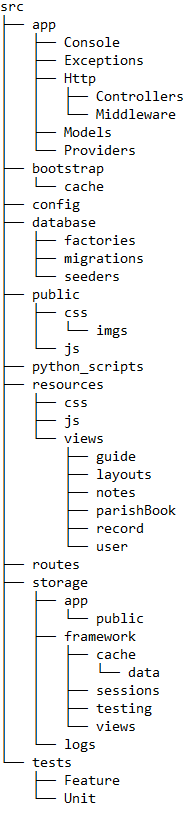
\includegraphics[width=37mm]{obrazky-figures/struktura.png}
	\caption[Adresářová struktura Laravel projetku]{Adresářová struktura Laravel projetku}
	\label{figure_structure}
\end{figure}

V~následujících kapitolách budou popsány implementace jednotlivých vrstev návrhového vzoru MVC v~rámci frameworku Laravel.
\subsection{Model}
Model v~Laravel frameworku z~většiny případů zastupuje databázovou tabulku, proto modely už v~základu dědí z~třídy \verb|Model|, která obsahuje proměnné pro definování různých atributů a hodnot, a zároveň nám poskytuje objektově relační mapování pro práci s~databází. Navíc můžeme vytvářet testovací data pro pomocí tzv. továrny. To je také důvod, proč model již ze základu používá trait třídu HasFactory \cite{Laravel1}.

V~rámci naší aplikace byly vytvořeny modely pro všechny tabulky reprezentující entity. Jedná se tedy osm modelů. Tyto modely obsahují funkce pro získání vhodných/vyfiltrovaných záznamů z~databáze či generování obsahu v~kódu HTML. Základní metody například pro vyhledání záznamu pomocí primárního klíče nebylo potřeba implementovat, protože jak bylo zmíněno v~odstavci výše, každý z~našich modelů dědí od Laravel třídy \verb|Model| a ta tyto metody poskytuje (například metoda \verb|find|). Metody těchto modelů jsou pak volané v~kontrolerech (viz kapitola \ref{controller}). Asi nejdůležitějším modelem je model \verb|Record|. Obsahuje totiž metody pro paginaci záznamů, generování kartiček a nebo pro získání matrik k~jednotlivým záznamům.

\subsubsection{Generování HTML kódu}
Jak bylo zmíněno výše modely obsahují metody pro generování kódu ve značkovacím jazyce HTML. Tyto metody jsou potřeba kvůli asynchronním požadavkům, kdy je zapotřebí dynamicky zobrazit uživateli elementy naplněné daty z~databáze. Ke každé operaci týkající se nějakého objektu databáze tak existuje metoda, která je schopná vygenerovat elementy a naplnit je daty objektu, které je potřeba zobrazit. Většinou se jedná o~statické metody náležící modelům příslušným k~danému objektu. Tyto metody zapisují kód formou řetězce, který je pak výstupem samotných metod. Řetězec je poté vložen do html prostřednictvím funkce \verb|.html()| z~knihovny jQuery. Tato funkce vloží do elementu, nad kterým je volaná, kód HTML, který je funkci předán jako řetězec.

\subsection{View}
Jedná se o~vrstvu, která slouží k~zobrazování dat uživateli. Obsahuje Blade šablony (s~HTML kódem). Blade je šablonovací systém, který na rozdíl od ostatních systémů nezakazuje používání PHP kódu v~pohledu, tudíž neslouží pouze pro vkládání proměnných do HTML kódu. Blade používá speciální syntaxi, jež je poté převedena na normální PHP kód, a zároveň tento vygenerovaný pohled je následně uložen do mezipaměti pro příští použití kvůli rychlejšímu načítání (pokud není daný pohled modifikován) \cite{Laravel2}.

Naše aplikace kromě základních uvítacích a autentizačních pohledů nabízí tři hlavní pohledy. V~následujících podkapitolách budou tyto pohledy podrobně popsány.

\subsubsection{Hlavní pohled}
Prvním pohledem, který uživatel uvidí po přihlášení je hlavní stránka (viz obrázek \ref{figure_main_page}). Na této stránce uživatel vidí všechny své doposud nahrané soubory prostřednictvím datové tabulky, kterou poskytuje knihovna jQuery. V~rámci této tabulky může uživatel vyhledávat soubory na základě jména či je řadit podle data nahrání. Další možností nabízenou uživateli v~rámci tabulky je mazání těchto souborů za pomocí malé červené ikonky. K~následkům této operace je uživatel upozorněn vyskakovacím oknem.

\begin{figure}[H]
	\centering
	\includegraphics[width=145mm]{obrazky-figures/main\_page.png}
	\caption[Hlavní stránka aplikace]{Hlavní stránka aplikace}
	\label{figure_main_page}
\end{figure}

Další akcí, kterou uživatel může provést na hlavní stránce, je přidání souboru. Učiní tak pomocí zeleného tlačítka "Přidat soubor"\ vyskytujícího se v~úrovni nadpisu stránky. Po stisknutí tlačítka se zobrazí vyskakovací okno, v~rámci kterého může uživatel vybrat soubor, který chce nahrát (viz obrázek \ref{figure_file_upload}). Prostřednictvím toho okna si může pro daný soubor uživatel také nastavit parametry výpočtu časových rozsahů (viz časové rozsahy v~kapitole~\ref{matcher}).

\begin{figure}[H]
	\centering
	\includegraphics[width=90mm]{obrazky-figures/file\_upload.png}
	\caption[Modalové okno pro nahrání souboru]{Modalové okno pro nahrání souboru}
	\label{figure_file_upload}
\end{figure}


Po nahrání souboru musí uživatel vyčkat až parser dokončí svou práci. Na aktivitu jiné komponenty je uživatel upozorněn pomocí načítacího kolečka. Během celého procesu nahrávání i zpracování souboru se uživatel pohybuje v~dříve zmíněném vyskakovacím okně. Po dokončení parseru je uživatel vybídnut ke zkontrolování přiřazených území a k~případnému doplnění území nepřiřazených (viz obrázek \ref{figure_suggestion}). 

\begin{figure}[H]
	\centering
	\includegraphics[width=85mm]{obrazky-figures/suggestions\_modal.png}
	\caption[Modalové okno pro kontrolu a doplnění území]{Modalové okno pro kontrolu a doplnění území}
	\label{figure_suggestion}
\end{figure}

Pro každé území je za pomocí bootstrapových komponent vytvořena rozbalovací kartička, ve které se nachází pole pro zadání území. Uživatel má buďto možnost si vybrat z~navržených území, nebo se pokusit území najít sám pomocí textového pole. Textové pole využívá komponenty jQueryUI autocomplete\footnote{autocomplete - automatické doplnění}, která uživateli na základě podobnosti k~psanému textu navrhuje území z~databáze. Jestliže uživatel, žádné území nevybere, nebo nějakou operací zadané území znevalidní, pak je pole označeno oranžovou barvou. Pro případy, že by uživatel chtěl území nastavit pro jednotlivé osoby/rodiny pak tak může provést za pomocí ozubeného kolečka kdy se mu zjeví stejné dříve zmíněné vstupní pole, které ovšem upravuje pouze individuální osobu/rodinu.

Po dokončení specifikace území je pak spuštěn matcher, který naváže matriky na záznamy. Během této operace uživatel opět vyčkává v~prostředí vyskakovacího okna. Po dokončení je pak přesměrován na pohled daného souboru.

\subsubsection{Stránka souboru}
Tato stránka zobrazuje uživateli jednotlivé záznamy vytvořené v~rámci rozkliknutého souboru (obrázek \ref{figure_record_page}). Záznamy jsou zobrazeny podle jejich typů. Uživatel si typ může změnit pomocí menu dostupného na vrcholu stránky. Zde se také vyskytuje vstupní pole, které slouží k~vyhledávání konkrétních záznamů pomocí ID osoby/rodiny. Vyhledávat lze také pomocí jména, a to i v~případě záznamu oddání, kdy se zobrazí záznamy, kde alespoň jeden z~svatebčanů má jméno podobné tomu zadanému. 

\begin{figure}[H]
	\centering
	\includegraphics[width=140mm]{obrazky-figures/record\_page.png}
	\caption[Pohled zobrazující záznamy]{Pohled zobrazující záznamy vytvořené k~souboru Tyl.ged}
	\label{figure_record_page}
\end{figure}

Pro každý záznam je vytvořena boostrapová kartička, která obsahuje základní informace o~osobě/rodině, které se záznam týká (obrázek \ref{figure_card}). Informace, jenž chybí jsou pak v~této kartičce zvýrazněny červeně. V~případě, že uživatel chce zahodit vytvořený záznam, může tak učinit pomocí červeného křížku. V~rámci této kartičky má uživatel možnost si zobrazit navržené matriky pomocí rozbalovacího tlačítka "Zobrazit matriky".

\begin{figure}[H]
	\centering
	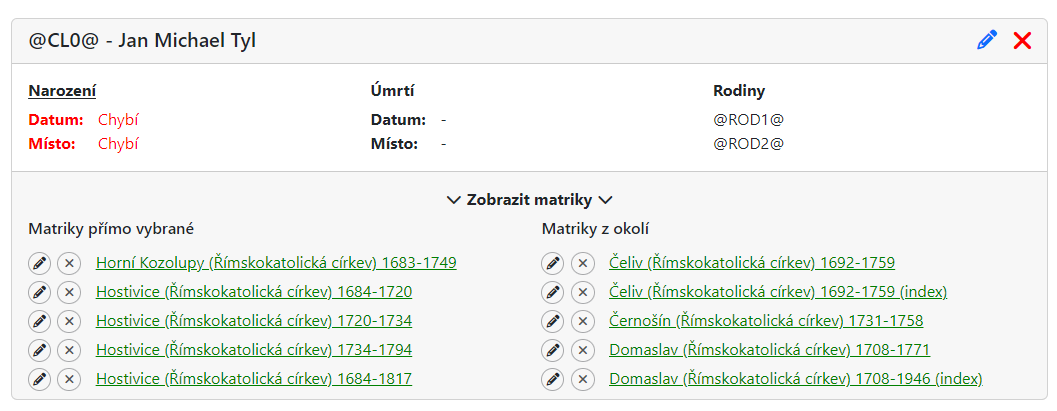
\includegraphics[width=140mm]{obrazky-figures/cards.png}
	\caption[Záznam pro událost narození reprezentovaný kartičkou]{Záznam pro událost narození reprezentovaný kartičkou pro osobu Jan Michael Tyl. V~obrázku jsou zobrazeny i matriky navržené pro tento záznam.}
	\label{figure_card}
\end{figure}

Matriky jsou zobrazeny ve dvou sloupcích. Levý sloupec představuje matriky vybrané přímo z~míst nalezených u~dané osoby, rodiny či příbuzných. V~pravém sloupci jsou pak matriky vybrané ze sousedních míst v~okolí 5 km. Matriky jsou řazeny podle priority relevance (viz sekce lokalit v~kapitole \ref{matcher}) a barevně odlišeny na základě této priority. Zobrazuje se vždy pouze pět matrik s~nejvyšší prioritou. Matriku je možné zahodit za pomocí křížku, a tato zahozená matrika pak bude nahrazena další, za předpokladu, že nějaká další je.

Kartičky se zobrazují na stránce v~omezeném množství. Zobrazit si další sadu kartiček uživatel může pomocí šipek vyskytujících se jak na vrchní tak spodní části stránky.

\subsubsection{Poznámky}
Další důležitou funkcionalitou aplikace je možnost zapisovat si poznámky k~osobám, rodinám a matrikám. Tato možnost je uživateli nabízena buďto v~záhlaví kartičky záznamu v~případě osob/rodin, anebo v~případě matrik hned vedle jejich výpisů. Poznámky jsou označeny pomocí ikonky tužky. Po kliknutí na tuto ikonku se vytvoří poznámka a zobrazí se modální okno (viz obrázek \ref{figure_note}). Prostřednictvím tohoto okna může uživatel upravit a uložit poznámku.

U~poznámek pro osobu/rodinu se nabízí možnost přidat matriku a psát poznámku k~této matrice. Pokud je pak zobrazena poznámka pro tuto matriku zobrazuje se v~ní i osoba/rodina, ve které je tato matrika zmíněna a také jejich sdílený text. Stejně tomu tak je s~přidáváním osob/rodin k~poznámce matriky.

\begin{figure}[H]
	\centering
	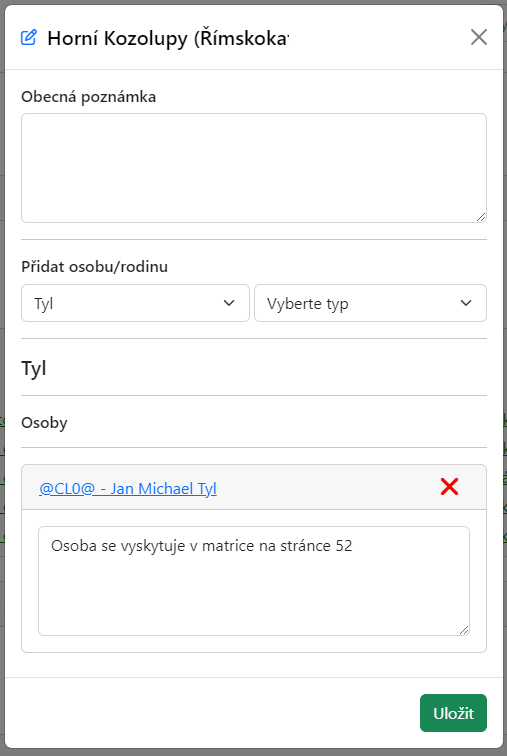
\includegraphics[width=80mm]{obrazky-figures/poznamka.png}
	\caption[Modalové okno zobrazující poznámku]{Modalové okno zobrazující poznámku k~matrice pocházející z~Horních Kozolup. Tato poznámka je propojená s~poznámkou k~osobě Jan Michael Tyl ze souboru Tyl.ged.}
	\label{figure_note}
\end{figure}

\subsubsection{Stránka poznámek}
Jedná se o~poslední pohled, který slouží k~zobrazení poznámek na jednom místě. Poznámky jsou zde zobrazeny pomocí tabulek a jsou rozděleny do tří tabulek podle jejich typů (osoba, rodina, matrika). Výběr typu se dá provést pomocí stejného menu použitého u~záznamů. V~tabulkách se dá poznámky, stejně jako na hlavní stránce u~souborů, vyhledávat za pomocí různých parametrů a nebo je řadit. Po kliknutí na řádek tabulky se poznámka rozevře a je možné ji tedy editovat i na této stránce.

\subsection{Controller}
\label{controller}
Kontroler je část, se kterou komunikuje uživatel. Předá jí parametry a ona mu vrátí data (např. HTML stránku). Kontroler typicky parametry předá modelům, od kterých získá data. Tato data předá pohledům (šablonám), které data začlení do nějakého HTML kódu. Tento HTML kód pošle kontroler uživateli do prohlížeče. Funguje tedy jako takový prostředník~\cite{Laravel2}.

Pro aplikaci byl ke každému modelu vytvořen jeho příslušný kontroler. Metody těchto kontrolerů jsou volány prostřednictvím routovacího souboru. Pro každou uživatelskou akci existuje metoda nějakého kontroleru, který tuto akci zpracovává, získává data z~příslušných modelů a předává je zpátky do pohledu na zobrazení. Metody jsou volány v~pohledech přes jejich adekvátní routy, kdy každá routa má své pojmenování. Volány jsou buďto synchronně v~případě přechodů mezi stránkami nebo asynchronně pomocí AJAXu, pokud se jedná o~nějakou operaci na stránce. Jestliže kontroler přijímá synchronní požadavek, pak vrací načtení celých pohledů. Pokud je požadavek asynchronní, pak vrací pouze potřebné proměnné, či modelem vygenerované elementy v~HTML kódu, a to prostřednictvím formátu JSON. V~následujících podkapitolách budou popsány způsoby, jakými kontrolery řeší některé důležité operace.

\subsubsection{Nahrání souboru}
O~nahrání, ale i smazání souboru se stará \verb|GFileController|. Operace nahrání souboru se vykonává pomocí asynchronních požadavků a skládá se z~několika kroků.

Nejdříve je pomocí metody \verb|store| zkontrolován uživatelem nahraný soubor. Pokud soubor není v~pořádku, pak metoda vrací chybovou hlášku, která je uživateli zobrazena. V~opačném případě je soubor dočasně nahrán na server a uložen do databáze společně s~hodnotami pro výpočty rozsahů, které mohl uživatel upravit.

Dalším krokem je spuštění parseru. O~tento krok se stará metoda \verb|executeParser|, která spouští skript a předává mu cestu k~nahranému souboru. Metoda pak vyčká na skončení parseru a přijímá od něj výsledek ve formátu JSON. Následně volá metodu modelu \verb|GFile|, která vygeneruje pro získaný výsledek kód v~HTML tak, aby jej bylo možné uživateli zobrazit. Výsledkem je v~tomto případě modalové okno pro kontrolu a doplnění území.

Posledním krokem, který \verb|GFileController| provádí je spuštění matcheru. Ten se spouští po zkontrolování/doplnění území pomocí metody \verb|executeMatcher|. Metoda vrací zprávu o~úspěšném ukončení skriptu. Přesměrování na detail souboru se už pak provádí prostřednictvím jiného kontroleru, tím je \verb|RecordController|.

Při nahrávání souboru se používá ještě \verb|TerritoryController|. Ten obsahuje hlavně metody sloužící k~načítání území při vyhledávání v~autocomplete poli, a nebo pak metodu \verb|assignTerritories|, která přiřadí doplněné území k~příslušným osobám/rodinám.

\subsubsection{Zobrazení záznamů}
O~veškeré operace ohledně záznamů se stará \verb|RecordController|. Synchronní načtení záznamů k~nějakému souboru provádí metoda \verb|index|. Tato metoda načte pohled starající se o~zobrazení záznamů a předá mu veškeré potřebné parametry. Asynchronní načtení se provádí pomocí metody \verb|get_records|. V~obou případech je využíváno metod modelu \verb|Record| pro získání záznamů či generování HTML obsahu. Asynchronní metoda nenačítá celou stránku, ale pouze získává nové kartičky záznamů na zobrazení. Asynchronní načítání záznamů se provádí při paginaci, vyhledávání pomocí tagu/jména, nebo mazání záznamu.

\verb|RecordController| se také stará o~procházení skrz navržené matriky. Tedy zahození návrhu pomocí křížku a zobrazení dalšího v~pořadí. Tento proces je obstaráván metodou \verb|delete_book_suggestion|, která vymaže návrh matriky pro daný záznam z~propojovací tabulky a načte nové knížky. K~tomu kontroler opět využívá metod modelu \verb|Record|. Tato metoda vrací nově vygenerovaný HTML kód pro zobrazení navržených knih.

\subsubsection{Vytvoření poznámky}
U~poznámek se ke zpracování požadavků používají celkově 4 kontrolery. \verb|NoteController| je ten hlavní, který se stará o~základní operace týkající se poznámek. Tedy zobrazení, vytvoření a aktualizace poznámek. Poznámka k~záznamu nebo matrice se vytváří až při kliknutí na ikonu tužky. Nejdříve \verb|NoteController| zkontroluje, zdali poznámka existuje pomocí metody \verb|check_if_exists|. Kontrola na existenci je důležitá, protože ikona tužky neslouží
pouze k~vytvoření poznámky, ale také k~zobrazení již existující.

Jestliže poznámka neexistuje, pak je vytvořena pomocí metody \verb|store|. Tato metoda na základě vstupních parametrů vyhodnotí ke komu má být poznámka napsána (osoba, rodina, matrika), tedy na koho bude v~databázi odkazovat cizím klíčem. Jméno poznámky se při vytváření generuje automaticky, a to podle toho, komu patří. Poté je poznámka přidána do databáze a může být zobrazena.

O~zobrazení poznámky se stará metoda \verb|fetch|. Kromě získání patřičného záznamu z~databáze získává tato metoda také všechny přidružené objekty k~této poznámce. Tedy osoby, rodiny nebo knížky, které si uživatel mohl k~poznámce přidat. U~těchto objektů je zapotřebí dynamicky generovat HTML kód a k~tomu se využívá funkcí modelu \verb|Note|. Tato funkce tedy vrací jak proměnné, které budou vsazeny do statického HTML kódu, tak dynamicky vygenerovaný HTML kód.

Poslední operací, o~kterou se \verb|NoteController| stará je aktualizace poznámky. Metoda \verb|update| aktualizuje jméno a textový obsah poznámky, ale také textový obsah všech přidaným objektů. Tato operace je vyvolána po použití tlačítka "Uložit".

Jak bylo zmíněno výše, k~poznámkám je možné přidávat objekty, ke kterým si uživatel může připisovat další text. Jestliže je poznámka vedena pro matriku, pak uživatel může k~poznámce přidat osoby a rodiny. V~opačném případě je možné přidat k~poznámce matriku. Pro jednotlivý typ objektu, který je možné přidat, jsou implementované metody kontrolerů \verb|PersonController|, \verb|FamilyController|, \verb|ParishBookController|. Pro zpřístupnění hledané osoby/rodiny/matriky existuje metoda \verb|get_person/family/parish_book|\footnote{Dále referencované jako "název\_object"}, která vrací vyhovující záznamy na zobrazení. Pro přidání je pak metoda \verb|add_object|, jež připojí objekt k~poznámce skrze propojovací tabulku. Poslední metodou je \verb|delete_object|, která odpojí objekt od poznámky vymazáním záznamu z~propojovací tabulky. Dvě poslední uvedené metody vrací nově vygenerovaný HTML kód obsahující nové rozpoložení připojených objektů. Tento kód opět generují metody modelu \verb|Note|.

\subsubsection{Uživatelské operace}
O~veškeré uživatelské operace jako jsou registrace, přihlášení, editace profilu a odhlášení se stará \verb|UserController|. Tento kontroler pracuje hlavně s~komponenty Laravelu pro autentizaci, třída \verb|Auth|, a udržení sezení, metoda \verb|session| patřící pod třídu \verb|Request|.

